\documentclass[11pt]{My_preprint}

\title{
    Buoyancy driven motion of non-coalescing inertial drops: 
    analysis and modeling of the microstructure kinematics. 
    %with nearest particle statistics. 
}

\author[1,2]{Nicolas Fintzi}
\author[1]{Jean-Lou Pierson}
\author[2]{Stephane Popinet}
\affil[1]{IFP Energies Nouvelles, Rond-point de l’echangeur de Solaize, 69360 Solaize}
\affil[2]{Sorbonne Universit\'e, Institut Jean le Rond d'Alembert, 4 place Jussieu, 75252 PARIS CEDEX 05, France}
\normalmarginpar


\begin{document}

\maketitle

\begin{abstract}
    In this study, we provide a comprehensive analysis of the timescale that govern the droplets' interaction as well as the global microstructure in buoyant emulsions. 
    It is shown  in \citep{fintzi2024buoyancy} that as predicted by \citet{zhang2023evolution}, the second moment of the nearest particle pair distribution, noted \textbf{R}, has the capability to quantify microstructure's features such as clusters and layers of particles.
    In this study we propose to analyze the microstructure kinematics   through the derivation of a transport equation for \textbf{R} within the framework of kinematics   theory. 
    We conducted Direct Numerical Simulations (DNS) of statistically steady state mono-disperse buoyant emulsion, over a broad range of \textit{Galileo} number ($Ga$), particle volume fraction ($\phi$), and viscosity ratio ($\lambda$). 
    The density ratio and the \textit{Bond} number are kept constant, $\zeta = 1.11$ and  $Bo = 0.2$, respectively. 
    By a rigorous theoretical and numerical analysis we could show that :
    (1) the time of relaxation of $\textbf{R}(\textbf{x},t)$, is the mean age of interaction of the  nearest particles pairs $\tau_p(\textbf{x},t)$;
    (2) The particle normal approach velocity scale as $\tau_p n_p^{1/3}$ with $n_p$ the number density, and has also a relaxation time of $\tau_p$.
    (3) We could evaluate the different source terms in the transport equation for $\textbf{R}$ in terms of the dimensionless parameters. 
    Overall the mean time of interaction $\tau_p$ seem to be a crucial quantity in the modeling of the particle relative kinematics   of dispersed two phase flows. 
\end{abstract}

\section{Introduction}





\begin{enumerate}
    \item We use extensively averaged models in industry 
    \item These models necessitate closure laws. These closure laws are highly dependent on the particles' microstructure. 
    \item In our previous work we performed a \textit{Nearest-particle-statistics} analysis of the microstructure geometry, or the steady state microstructure. 
    \item All the closures in the literature are performed in steady state system. 
    Therefore, in order to be valid in a Euler-Euler averaged context the time scales of the simulation must be greater than the time for the microstructure to reach its steady state. 
    Only then the assumption of quasi steady ness is valid.    
    \item Therefore, in this study we provide a theoritical and numerical analyssi of the timescale that drives the microstructure. 
    Doing so, we demonstrate that the particle interaction time is the main timescale involved in the microstructure relaxation time. 
    We therefor also study the relative kinematic
\end{enumerate}

% \subsection{Numerical method}

In this problem, the governing equations consist of the one-fluid formulation of the mass and momentum equation, with an additional transport equation for the dispersed phase indicator function. 
We recall their form here, 
\begin{align}
    \pddt \rho+ \div(\rho\textbf{u})
    &= 0,\\
    \label{eq:dt_urho}
    \pddt (\rho \textbf{u})
    + \div (\rho  \textbf{u} \textbf{u} - \bm\sigma)
    &= (\avg{\rho} - \rho)\textbf{g}
    + \textbf{f}_\gamma,\\
    \label{eq:dt_C}
    \pddt C + \textbf{u}\cdot\grad C  
    &= 0,
\end{align}
% \tb{mettre le link navier stokes solver et faire ca pour le reste }
which are the mass, momentum and colors function transport equation, respectively. 
The scalar fields $C$, represents the color function, which range between $0$ and $1$ to indicate the proportion of fluid and dispersed phase, respectively. 
We introduced the fluid velocity vector $\textbf{u}$ and the Newtonian stress tensor $\bm{\sigma} = -p \textbf{I} + \mu (\grad \textbf{u}+ \grad \textbf{u}^\dagger)$ where $p$ is the pressure fields and $^\dagger$ represents the transpose operator.
Note that the material properties, $\rho$ and $\mu$, take the value of the phases in presence, following the arithmetic average : $\rho = (1-C)\rho_f + C \rho_d$ and $\mu = (1-C)\mu_f + C \mu_d$. 
In our case the arithmetic mean turns out to perform better compared to the harmonic mean, which is often used to interpolate the viscosity for bubbly flows \citet{hidman2023assessing,innocenti2020direct}.
More details about this choice is provided in \ref{ap:validation} (\textit{Case 1.}). 
The capillary force is defined as, $\textbf{f}_\gamma =\textbf{n} \gamma \div \textbf{n} $, where \textbf{n} is the normal at the interface.
Following  \citep{bunner2002dynamics}, we incorporated the artificial body force term, $\avg{\rho}\textbf{g}$, on the right-hand side of \ref{eq:dt_urho}, to maintain a zero-averaged velocity throughout the entire numerical domain.  

To solve these equations we first initialized $125$ spherical droplets within a cubic domain with fully periodic boundary condition. 
We used the open source code \url{http///basilisk.fr} to discretize the governing equations in a multigrid solver. 
The Navier-Stokes equations are discretized with a centered scheme.
The two-phase flow solver uses the Volume of Fluid (VoF) method. 
The interfaces between the droplets and the carrier fluid is reconstructed using the Piecewise Linear Inter-face Calculation or PLIC method \citet[Chapter 5.]{tryggvason2011direct}.
Regarding the treatment of the surface tension force term we refer the reader to \citet{popinet2018numerical} for more details. 
The Basilisk solver has been validated extensively, in the framework of bubbly flow. 
Most of the previous studies \citep{hidman2023assessing,innocenti2020direct} recommend a grid definition of $\Delta/d \ge  30$, where $\Delta$ is the grid spacing. 
In \ref{ap:validation} we carried a mesh independence study and demonstrate that a grid spacing of $\Delta = d/30$ is also suitable in our context.
For readers seeking more detailed information about the solvers, we recommend the wiki pages : \href{http://basilisk.fr/src/navier-stokes/centered.h}{centered.h}, \href{http://basilisk.fr/src/tension.h}{tension.h} and \href{http://basilisk.fr/src/poissson.h}{poissson.h} where he can find the source code of the Navier-Stokes, surface tension and multigrid solver used in this work, respectively. 

With the VoF method droplets and bubbles may experience premature coalesce.
For a detailed discussion on this issue, see  \citet[Appendix B]{innocenti2020direct}.
However, in this work, it is imperative to conserve a specific (mono-disperse) population of droplets over time to accumulate sufficient statistics about the microstructure.
To tackle this issue we present in the next section a novel algorithm which prevent coalescence between droplets, while maintaining a reasonable cost. 







\section{Theoretical framework}
\label{sec:Theory}
In the preceding chapter we have seen that the granular temperature could be estimated based on the vector
\begin{equation*}
    \textbf{u}^\text{nst}_p (\textbf{x},\textbf{r},t,a)
    = 
    \frac{1}{P_{nst}(\textbf{x},\textbf{r},t,a)}
    \int \sum_{i}^{N_b}\delta(\textbf{x}-\textbf{x}_i)
    \sum_{j\neq i}^{N_b}\delta(\textbf{x}+\textbf{r}-\textbf{x}_j) 
    \delta(t+a-t_c^{ij}) 
    \textbf{u}_{ij}
    h_{ij} 
    d\mathscr{P}.
    \label{eq:q_nstij}
\end{equation*}
the aim of this chapter is therefore to determine the form of $\textbf{u}^\text{nst}_p$. 

In addition to provides physical explanation the field $\textbf{u}_p^d = \textbf{u}^r_p - \textbf{u}_p$ is of great importance to study the particle phase fluctuation tensor $\avg{\delta_i \textbf{u}_i' \textbf{u}_i'}$ which is of crucial importance in multiphase flow modeling. 
Indeed, it can be shown that 
\begin{equation*}
    \frac{\avg{\delta_i \textbf{u}_i' \textbf{u}_i'}}{n_p}(\textbf{x},t)
    =  
    \int_{\mathbb{R}^3 }
    \textbf{u}_p^d
    \textbf{u}_p^d
    P_{nst}(\textbf{r}|\textbf{x},t)
    d\textbf{r}
    + \int_{\mathbb{R}^3 }
    \textbf{F}(\textbf{r},\textbf{x},t)
    d\textbf{r}
\end{equation*}
where, $\textbf{F} = \avg{\sum_i\sum_{j\neq i}\delta_j\delta_i h_{ij}(\textbf{u}_i - \textbf{u}_p^{nst})(\textbf{u}_i - \textbf{u}_p^{nst})}$. 
Thus, the ensemble averaged particle phase Reynolds stress is the sum of the fluctuation given by $\textbf{u}_p^r$ plus an additional contribution form the others particles fluctuation around the average field $\textbf{u}_p^d$. 


\section{A transport equation for the nearest particle velocity-included pdf properties}

We propose an alternative derivation, to what it is done in \citet{zhang2023evolution} for the derivation of the nearest particle averaged properties. 



The derivation is done by noticing that at the local level we have, 
\begin{align*}
    \pddt \delta(\textbf{x}_i(\FF,t) - \textbf{x})
    + \textbf{u}_i(\FF,t) \cdot \pddx \delta(\textbf{x}_i(\FF,t) - \textbf{x})
    = 0\\
    \pddt \delta(\textbf{u}_i(\FF,t) - \textbf{u})
    + \textbf{a}_i(\FF,t) \cdot \pddu \delta(\textbf{u}_i(\FF,t) - \textbf{u})
    = 0\\
    \pddt \delta(\textbf{x}_j(\FF,t) - \textbf{x}+\textbf{r})
    + \textbf{w}_{ji}(\FF,t) \cdot \pddr \delta(\textbf{x}_j(\FF,t) - \textbf{x}+\textbf{r})
    + \textbf{u}_{i}(\FF,t) \cdot \pddr \delta(\textbf{x}_j(\FF,t) - \textbf{x}+\textbf{r})
    = 0\\
    \pddt \delta(t+a - t^{ij}_c(\FF))
    - \pdda \delta(t+a - t^{ij}_c(\FF))
    = 0,
\end{align*}
where we have defined $\textbf{w}_{ji} = \textbf{u}_j - \textbf{u}_i$ as the relative velocity between particle $j$ and $i$, and $\pddt \textbf{u}_i = \textbf{a}_i$ as the acceleration of the particle . 
For clearly, we note what we call here the \textit{state} function $\Pi$ as, 
\begin{equation*}
    \Pi(\textbf{x},\textbf{r},\textbf{u},t,a,\FF)
    = 
    \sum_i 
    \delta(\textbf{x}_i(\FF,t) - \textbf{x})
    \delta(\textbf{u}_i(\FF,t) - \textbf{u})
    \sum_{j\neq i}\delta(\textbf{x}_j(\FF,t) - \textbf{x}+\textbf{r})
    \delta(t+a - t^{ij}_c(\FF))
    h_{ij}(t,\FF)
\end{equation*}
Then, one may directly deduce that, $\Pi$ follows the conservation equation, 
\begin{equation}
    \pddt \Pi 
    + \pdda \Pi 
    + \pddx\cdot(\textbf{u}_i \Pi)
    + \pddu\cdot(\textbf{a}_{i} \Pi)
    + \pddr\cdot(\textbf{w}_{ji} \Pi)
    = 
    \Pi_S
    \label{eq:dt_Pi}
\end{equation}
where the source term is explicitly defined by, 
\begin{align*}
    \Pi_S
    &= 
    \sum_i 
    \delta(\textbf{x}_i(\FF,t) - \textbf{x})
    \delta(\textbf{u}_i(\FF,t) - \textbf{u})
    \sum_{j\neq i}\delta(\textbf{x}_j(\FF,t) - \textbf{x}-\textbf{r})\\
    &\delta(t+a - t^{ij}_c(\FF))
    h_{ij}(t,\FF)
    \sum_{l\neq i} 
    \delta(r_{li} - r_{jl})
    (\textbf{n}_{li}\cdot\textbf{u}_{li}
     - \textbf{n}_{ji}\cdot \textbf{u}_{ji})\\
    &= 
    \Pi
    \sum_{l\neq i} 
    \delta(r_{li} - r_{jl})
    (\textbf{n}_{li}\cdot\textbf{u}_{li}
     - \textbf{n}_{ji}\cdot \textbf{u}_{ji})\\
\end{align*}
such that 
\begin{align*}
    \iiint \Pi_S  d\PP dS(\textbf{r}) da =
    \iint [\delta(a)P(\textbf{x},\textbf{r},\textbf{u},t,0)
    - \frac{P_\text{nst}(\textbf{x},\textbf{r},,\textbf{u}t,a)}{\tau^\text{nst}(\textbf{x},\textbf{r},\textbf{u},t,a)}] dS(\textbf{r}) da
    = 0 
\end{align*}
is a source terms related to the inter-changes in nearest neighbors. 

Firstly, notice that integrating \ref{eq:dt_Pi} on all configurations yields the same conservation equation as \citet{zhang2023evolution} for $P_\text{nst}$. 
Making our derivation consistent with his. 


To derive an equation for $\textbf{u}_p^\text{nst}$ the process is easy, 
we simply multiply \ref{eq:dt_Pi} by $\textbf{u}_i$ and average on all configurations. 
It yields, 
\begin{equation*}
    \pddt \avg{\Pi \textbf{u}_i}
    + \pdda \avg{\Pi  \textbf{u}_i}
    + \pddx\cdot\avg{\textbf{u}_i \textbf{u}_i  \Pi}
    + \pddu\cdot\avg{\textbf{a}_i \textbf{u}_i  \Pi}
    + \pddr\cdot \avg{ \textbf{u}_i \textbf{w}_{ji} \Pi}
    = 
    \avg{\Pi_S \textbf{u}_i}
    + \avg{\Pi \textbf{a}_i }
\end{equation*}
Noticing that, $\avg{\textbf{u}_i \Pi} = \textbf{u}P_\text{nst}$ we directly obtain the equation for \textbf{u}:
\begin{multline*}
    \pddt (\textbf{u} P_\text{nst})
    + \pdda (\textbf{u} P_\text{nst})
    + \pddx \cdot  (\textbf{u} \textbf{u}  P_\text{nst})
    + \pddr \cdot  (\textbf{u}\textbf{w}^\text{nst}_p P_\text{nst})
    + \pddu \cdot  (\textbf{u}\textbf{a}^\text{nst}_p P_\text{nst})\\
    = \textbf{u} 
    \left[\delta(a)  P(\textbf{x},\textbf{r}, \textbf{u},t,0)
    - \frac{P_\text{nst}(\textbf{x},\textbf{r},\textbf{u},t,a)}{\tau^\text{nst}(\textbf{x},\textbf{r},\textbf{u},t,a)}
    \right]
    + \textbf{a}_p^\text{nst}
    P_\text{nst} 
\end{multline*}


With our new notation we have shown that we have the exact notation, 
\begin{equation*}
    \avg{\delta_i \textbf{u}_i' \textbf{u}_i'}
    = 
    \int 
    \textbf{uu}
    P_\text{nst}(\textbf{x},\textbf{r},\textbf{u},a,t)
    d\textbf{r}
    d\textbf{u}
    da
    - \textbf{u}_p \textbf{u}_p n_p
\end{equation*}
Thus, we rather derive the previous equation by \textbf{u} which gives, 
\begin{multline*}
    \pddt (\textbf{uu} P_\text{nst})
    + \pdda (\textbf{uu} P_\text{nst})
    + \pddx \cdot  (\textbf{uu} \textbf{u}  P_\text{nst})
    + \pddr \cdot  (\textbf{uu}\textbf{w}^\text{nst}_p P_\text{nst})
    + \pddu \cdot  (\textbf{uu}\textbf{a}^\text{nst}_p P_\text{nst})\\
    = \textbf{uu} 
    \left[\delta(a)  P(\textbf{x},\textbf{r}, \textbf{u},t,0)
    - \frac{P_\text{nst}(\textbf{x},\textbf{r},\textbf{u},t,a)}{\tau^\text{nst}(\textbf{x},\textbf{r},\textbf{u},t,a)}
    \right]
    + \textbf{u}\textbf{a}_p^\text{nst}
    + \textbf{a}_p^\text{nst}\textbf{u}
    P_\text{nst} 
\end{multline*}
integrating Overall age and velocity and relative position gives, 
\begin{equation*}
    \pddt (n_p \textbf{F}_p )
    +\pddx (n_p\textbf{F}_p \textbf{u}_p  + n_p \textbf{F}^{Re})
    = 
    - \frac{n_p \textbf{F}_p }{\tau_p}
    + n_p \textbf{B}_p
    + n_p \textbf{D}_p
    + n_p \textbf{A}_p
\end{equation*}
with, 
\begin{align*}
    n_p \textbf{F}^{Re}(\textbf{x},t)
    =
    \int_{0}^\infty
    \int_{\mathbb{R}^6}
    \textbf{uu}(\textbf{u}- \textbf{u}_p)
    P(\textbf{x},\textbf{r},t,a)
    d\textbf{r}
    d\textbf{u}
    da,\\
    n_p \textbf{B}(\textbf{x},t)
    =
    \int_{0}^\infty
    \int_{\mathbb{R}^6}
    \textbf{uu}
    P(\textbf{x},\textbf{r},t,0)\delta(a)
    d\textbf{r}
    d\textbf{u}
    da, \\
    n_p\textbf{D}(\textbf{x},t) = 
    \int_{0}^\infty
    \int_{\mathbb{R}^6} \textbf{uu}
    \left[
        \frac{1}{\tau_p(\textbf{x},t)}
        - \frac{1}{\tau^\text{nst}(\textbf{x},\textbf{r},t,a)}
    \right]
    P_\text{nst}
    d\textbf{r}
    d\textbf{u}
    da,\\
    n_p \textbf{W}(\textbf{x},t) = 
    \int_{0}^\infty
    \int_{\mathbb{R}^6} \left[
        \textbf{u} \textbf{a}^\text{nst}_p
        + \textbf{a}^\text{nst}_p\textbf{u}
    \right]P_\text{nst}
    d\textbf{r}
    d\textbf{u}
    da.
\end{align*} 
Which is a global evolution equation for the particle tensor. 
However, notice how this is pointless since one may directly notice that, 
\begin{align*}
    \int\iiint \textbf{uu}\Pi_S  d\PP dS(\textbf{r}) da d\textbf{u} dr =
    \iint \textbf{uu} 
    \iint [\delta(a)P(\textbf{x},\textbf{r},\textbf{u},t,0)
    - \frac{P_\text{nst}(\textbf{x},\textbf{r},,\textbf{u}t,a)}{\tau^\text{nst}(\textbf{x},\textbf{r},\textbf{u},t,a)}] dS(\textbf{r}) da
    dr d \textbf{u}
    = 0 
\end{align*}
Indeed, since $\textbf{u}$ is not explicitly related to the particle relative position, this is not affected by this source term.. . 
And therefore, 
\begin{equation*}
    \pddt (n_p \textbf{F}_p )
    +\pddx (n_p\textbf{F}_p \textbf{u}_p  + n_p \textbf{F}^{Re})
    = 
    \int_{0}^\infty
    \int_{\mathbb{R}^6} \left[
        \textbf{u} \textbf{a}^\text{nst}_p
        + \textbf{a}^\text{nst}_p\textbf{u}
    \right]P_\text{nst}
    d\textbf{r}
    d\textbf{u}
    da.
\end{equation*}

\begin{figure}[h!]
    \centering
    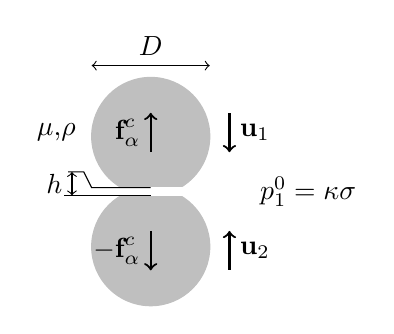
\begin{tikzpicture}
      \draw[lightgray,fill = lightgray] (0,0.7) circle (0.75);
      \draw[lightgray,fill = lightgray] (0,-0.7) circle (0.75);
      \draw[white,fill=white] (-0.75,-0.05) rectangle (0.75,0.05);
      \draw(0,0.05)--++(-0.75,0)--++(-0.1,0.2)--++(-0.2,0);
      \draw(0,-0.05)--++(-1.1,0);
      \draw[<->](-1,-0.05) --++ (0,0.3)node[midway,left]{$h$};
      \draw[<->](-0.75,1.6)--++(1.5,0)node[midway,above]{$D$};
      \node (para) at (-1.2,0.75){$\mu$,$\rho$};
      \node (pressure) at (2,0){$p_1^0 = \kappa \sigma$};
      \draw[->,thick](0,0.5)--++(0,0.5)node[midway,left]{$\textbf{f}_\alpha^\text{c}$};
      \draw[->,thick](0,-0.5)--++(0,-0.5)node[midway,left]{$-\textbf{f}_\alpha^\text{c}$};
      \draw[<-,thick](1,0.5)--++(0,0.5)node[midway,right]{$\textbf{u}_1$};
      \draw[<-,thick](1,-0.5)--++(0,-0.5)node[midway,right]{$\textbf{u}_2$};
    \end{tikzpicture}
    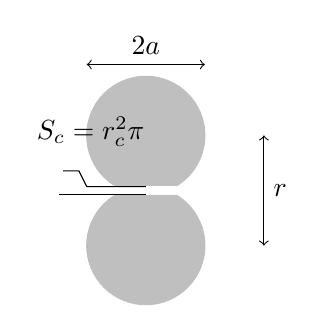
\begin{tikzpicture}
      \draw[lightgray,fill = lightgray] (0,0.7) circle (0.75);
      \draw[lightgray,fill = lightgray] (0,-0.7) circle (0.75);
      \draw[white,fill=white] (-0.75,-0.05) rectangle (0.75,0.05);
      \draw(0,0.05)--++(-0.75,0)--++(-0.1,0.2)--++(-0.2,0);
      \draw(0,-0.05)--++(-1.1,0);
      \draw[<->](-0.75,1.6)--++(1.5,0)node[midway,above]{$2 a$};
      \draw[<->](1.5,0.7)--++(0,-1.4)node[midway,right]{$r$};
      \node (para) at (-0.7,0.75){$S_c = r_c^2 \pi$};
    \end{tikzpicture}
    \caption{Scheme of two colliding droplets at close contact. Notice the null kurvature in the region of the interface close to the film leading to a capilary force $\textbf{f}_\alpha^\text{c} \approx - S_c \kappa \sigma \textbf{r}/|\textbf{r}|$. }
\end{figure}
the inter particle force 
\begin{equation*}
    \textbf{f}_{ij}^\text{c}
    = S_c \kappa \gamma \textbf{r}_{ij}/r_{ij}
    = \pi r_c^2 \kappa \gamma \textbf{r}_{ij}/r_{ij}
    = \pi (a^2 - r_{ij}^2/4) \kappa \gamma  \textbf{r}_{ij}/r_{ij}
\end{equation*} 
where the 
The resultants of these forces on the particle $i$ is therefore the sum of the contact with all particles except the $j^\text{th}$ particle, 
\begin{equation*}
    \textbf{f}_{i}^\text{c}
    = \sum_{j \neq i}\textbf{f}_{ij}
    = - \sum_{j \neq i} \pi (a^2 - r_{ij}^2/4) \kappa \gamma \textbf{r}_{ij}/r_{ij}
\end{equation*} 
The relative acceleration might be written as, 
\begin{equation*}
    a_p^\text{nst}
    = 
    \pi (a^2 - r^2/4) \kappa \gamma \textbf{r}/r
\end{equation*}
where we assume that the force is only due to the only nearest neighbor. 
Thus, 
\begin{equation*}
    \int_{0}^\infty
    \int_{\mathbb{R}^6} \left[
        \textbf{u} \textbf{a}^\text{nst}_p
    \right]P_\text{nst}
    d\textbf{r}
    d\textbf{u}
    da.
    = 
    \int_{0}^\infty
    \int_{\mathbb{R}^6} \left[
        \textbf{u} \pi (a^2/r - r/4) \kappa \gamma \textbf{r}
    \right]P_\text{nst}
    d\textbf{r}
    d\textbf{u}
    da
\end{equation*}


\subsection{Let remove the condition on $\textbf{u}_i$ for $\Pi$. }
It gives, 
\begin{equation*}
    \avg{\delta_i \textbf{u}_i' \textbf{u}_i'}(\textbf{x},t)
    =  
    \int_{\mathbb{R}^3 }
    (\textbf{u}_p^\text{nst} -\textbf{u}_p)
    (\textbf{u}_p^\text{nst} - \textbf{u}_p)
    P_{nst}(\textbf{r},\textbf{x},a,t)
    d\textbf{r}
    + \int_{\mathbb{R}^3 }
    \textbf{F}(\textbf{r},\textbf{x},t)
    d\textbf{r}
\end{equation*}
where, $\textbf{F} = \avg{\Pi (\textbf{u}_i - \textbf{u}_p^{nst})(\textbf{u}_i - \textbf{u}_p^{nst})}$. 

\begin{equation*}
    \pddt \avg{\Pi \textbf{u}_i}
    + \pdda \avg{\Pi  \textbf{u}_i}
    + \pddx\cdot\avg{\textbf{u}_i \textbf{u}_i  \Pi}
    + \pddr\cdot \avg{ \textbf{u}_i \textbf{w}_{ji} \Pi}
    = 
    \avg{\Pi_S \textbf{u}_i}
    + \avg{\Pi \textbf{a}_i }
\end{equation*}
which gives, 
\begin{multline*}
    \pddt (\textbf{u}_p^\text{nst} P_\text{nst})
    + \pdda (\textbf{u}_p^\text{nst} P_\text{nst})
    + \pddx \cdot  (\textbf{u}_p^\text{nst} \textbf{u}^\text{nst}  P_\text{nst} + \textbf{u}^{Re})
    + \pddr \cdot  (\textbf{u}_p^\text{nst} \textbf{w}^\text{nst}_p P_\text{nst}+ \textbf{w}^{Re})\\
    = \delta(a)  \textbf{u}_p^\text{nst} P(\textbf{x},\textbf{r}, \textbf{u},t,0)
    - \frac{ \textbf{u}_p^{nst}(|D) P_\text{nst}(\textbf{x},\textbf{r},\textbf{u},t,a)}{\tau^\text{nst}(\textbf{x},\textbf{r},\textbf{u},t,a)}
    + \textbf{a}_p^\text{nst}
    P_\text{nst} 
\end{multline*}

\subsection*{Model for the conditioned acceleration based on numerical results}
% \section{Mesoscale equations}

Let $\delta_i(\textbf{x},t) = \delta(\textbf{x} - \textbf{x}_i(t))$ with $\delta$ the Dirac function and $\textbf{x}_i$ the position of the particle $i$.  
Similarly, we define $\delta_j(\textbf{y},t) =\delta(\textbf{y} - \textbf{x}_j(t)) $ for the particle label $j$. 
Then, it is trivial to show that, 
\begin{align*}
    \pddt \delta_i + \partial_\textbf{x} \cdot (\textbf{u}_i \delta_i) &= 0\\
    \pddt \delta_j + \partial_\textbf{y} \cdot (\textbf{u}_j \delta_j) &= 0.
\end{align*}
where we introduced $\textbf{u} = \ddt \textbf{x}$
and both equation equal $0$ since we do not consider particle appearance or vanishing. 
Manipulating those equations we can then have, 
\begin{equation}
    \pddt (\delta_j\delta_i) + \partial_\textbf{x} \cdot (\textbf{u}_i \delta_i\delta_j) + \partial_\textbf{y} \cdot (\textbf{u}_j \delta_i\delta_j) = 0.
    \label{eq:delta_beta_delat_alpha}
\end{equation}
The pair distribution function is defined as,
\begin{equation}
    P_2(\textbf{x},\textbf{y}) = \int \sum_i\delta_i(\textbf{x},t) \sum_j\delta_j(\textbf{y},t) P(\mathscr{C})d\mathscr{C}
\end{equation}
and the conditional pair average of a quantity \textbf{q} is defined as, 
\begin{equation}
    \avg{\textbf{q}}_2(\textbf{x},\textbf{y})P_2(\textbf{x},\textbf{y}) = \int \sum_i\delta_i(\textbf{x},t) \sum_j\delta_j(\textbf{y},t) \textbf{q} P(\mathscr{C})d\mathscr{C}
\end{equation}
Therefore, summing \ref{eq:delta_beta_delat_alpha} over all $i$ and $j$ and integrating on every configuration gives, 
\begin{equation}
    \pddt P_2 + \partial_\textbf{x} \cdot (\condavg{\textbf{u}_i}{2}P_2) + \partial_\textbf{y} \cdot (\condavg{\textbf{u}_j}{2}P_2) = 0.
    \label{eq:P_2}
\end{equation}
where then obtain an evolution equation for $P_2(\textbf{x},\textbf{y},t)$
integrating \ref{eq:P_2} over $\textbf{y}$ would give us the classic number density equation. 

Now let's define 
\begin{equation*}
    h_{ij} 
    = \frac{1}{N_i}
    \prod_{k \neq i,j}
    H(|\textbf{x}_k - \textbf{x}_i| - |\textbf{x}_j - \textbf{x}_i|)
    = \frac{1}{N_i}
    \prod_{k \neq i,j}
    H_{kij}
\end{equation*}
\begin{equation*}
    N_i
    = 
    \sum_{j\neq i}
    \prod_{k \neq i,j}
    H(|\textbf{x}_k - \textbf{x}_i| - |\textbf{x}_j - \textbf{x}_i|)
    = 
    \sum_{j\neq i}
    \prod_{k \neq i,j}
    H_{kij}
\end{equation*}
The function $h_{ij} (\mathscr{C}) = 1/N_i$ , if particle $j$ is one
of the nearest neighbors to particle $i$ in configuration $\mathscr{C}$ ;
and $h_{ij} (\mathscr{C} ) = 0$ otherwise.

Multiplying \ref{eq:delta_beta_delat_alpha} by $h_{ij}$ gives, 
\begin{equation}
    \pddt (\delta_j\delta_i h_{ij}) + \partial_\textbf{x} \cdot (\textbf{u}_i \delta_i\delta_j h_{ij}) + \partial_\textbf{y} \cdot (\textbf{u}_j \delta_i\delta_j h_{ij}) = \delta_j\delta_i\pddt h_{ij}
    \label{eq:delta_beta_delat_alpha_h}
\end{equation}
Considering implicit summation on $i$ and $j$ and integrating equation \ref{eq:delta_beta_delat_alpha_h}  yields, 

\begin{multline}
    \pddt \left(\int \delta_j\delta_i h_{ij} d\mathscr{P} \right) 
    + \partial_\textbf{x} \cdot \left(\int\textbf{u}_i \delta_i\delta_j h_{ij} d\mathscr{P} \right) 
    + \partial_\textbf{y} \cdot \left( \int \textbf{u}_j \delta_i\delta_j h_{ij} d\mathscr{P} \right) 
    \\=\int \delta_j\delta_i\pddt h_{ij} \mathscr{P}
\end{multline}
defining $\nstavg{\textbf{u}_i} P_{nst}= \int\textbf{u}_i \delta_i\delta_j h_{ij} d\mathscr{P} $ and $P_{nst} = \int \delta_j\delta_i h_{ij} d\mathscr{P} $ we obtain :
\begin{equation}
    \pddt \left(P_{nst} \right) 
    + \partial_\textbf{x} \cdot \left(\nstavg{\textbf{u}_i} P_{nst}\right) 
    + \partial_\textbf{y} \cdot \left( \nstavg{\textbf{u}_j} P_{nst} \right) 
    =\int \delta_j\delta_i\pddt h_{ij} \mathscr{P}
\end{equation}

\subsection*{Computation of the kernel }
We now want to find the expression of $\pddt h$. 
\begin{align*}
    \pddt h_{ij}
    &= \pddt \left(
        \frac{1}{N_i}
    \right)
    \prod_{k \neq i,j}  H_{kij}
    + \frac{1}{N_i} \pddt \left[
        \prod_{k \neq i,j}
        H_{kij} 
    \right] \\
    &= - \frac{\pddt N_i}{N_i^2}
    \prod_{k \neq i,j}  H_{kij}
    + \frac{1}{N_i} \sum_{l \neq i,j} \left[
        \pddt H_{lij}
        \prod_{k \neq i,j,l}
        H_{kij} 
    \right] \\
\end{align*}
From now on we decompose the calculation. 
Notice that we need to derive $\pddt N_i$ which is, 
\begin{equation}
   \pddt N_i
    = 
    \sum_{j\neq i}
    \pddt
    \prod_{k \neq i,j}
    H_{kij}\\
    = \sum_{j\neq i}
    \sum_{l \neq i,j} \left[
        \pddt H_{lij}
        \prod_{k \neq i,j,l}
        H_{kij} 
    \right]
\end{equation}
Then we can imporove the notaition
\begin{multline}
    \pddt h_{ij}
    = \\
    - h_{ij} \frac{1}{N_i}
    \sum_{j\neq i}
    \sum_{l \neq i,j} \left[
        \pddt H_{lij}
        \prod_{k \neq i,j,l}
        H_{kij} 
    \right]
    + \frac{1}{N_i} \sum_{l \neq i,j} \left[
        \pddt H_{lij}
        \prod_{k \neq i,j,l}
        H_{kij} 
    \right] 
\end{multline}

Considering that 
\begin{equation*}
    \pddt H(|\textbf{x}_l - \textbf{x}_i| - |\textbf{x}_j - \textbf{x}_i|)
    = \left(
        \pddt|\textbf{x}_l - \textbf{x}_i| - \pddt|\textbf{x}_j - \textbf{x}_i|
    \right)
    \delta(|\textbf{x}_l - \textbf{x}_i| - |\textbf{x}_j - \textbf{x}_i|)
\end{equation*}
where we assumed that $\pddt H(x) = \delta(x)$, and if we take $\pddt |f(x)| = \frac{f(x) f'(x)}{|f(x)|}$
\begin{multline*}
    \pddt H(|\textbf{x}_l - \textbf{x}_i| - |\textbf{x}_j - \textbf{x}_i|)
    \\= 
    \left[
    \frac{(\textbf{x}_l - \textbf{x}_i) \cdot (\textbf{u}_l - \textbf{u}_i)}{|\textbf{x}_l - \textbf{x}_i|}
    - 
    \frac{(\textbf{x}_j - \textbf{x}_i) \cdot(\textbf{u}_j - \textbf{u}_i)}{|\textbf{x}_j - \textbf{x}_i|}
    \right]\delta(|\textbf{x}_l - \textbf{x}_i| - |\textbf{x}_j - \textbf{x}_i|)
    \\= 
    \left[
    \textbf{n}_{li}\cdot \textbf{w}_{li}
    - 
    \textbf{n}_{ji}\cdot\textbf{w}_{ji}
    \right]\delta(|\textbf{x}_l - \textbf{x}_i| - |\textbf{x}_j - \textbf{x}_i|)
    \\= U_{lij}\delta_{lij}
\end{multline*}
Therefore, $\pddt H$ is the difference between the relative velocities between the $j$ and $l$ with the particle $i$ particles along their relative position. 

Finally, 
\begin{multline}
    \pddt h_{ij}
    = 
   \frac{1}{N_i} \sum_{l \neq i,j} \left[
    U_{lij}
    \delta_{lij}
    \prod_{k \neq i,j,l}
    H_{kij} 
    \right] 
    -  \frac{h_{ij}}{N_i}
    \sum_{j\neq i}
    \sum_{l \neq i,j} \left[
        U_{lij}
        \delta_{lij}
        \prod_{k \neq i,j,l}
        H_{kij} 
    \right]
    \label{eq:dt_h_ij}
\end{multline}
To summary : 
\begin{itemize}
    \item $H_{kij} =  1$ if $|\textbf{x}_k - \textbf{x}_i| > |\textbf{x}_j - \textbf{x}_i|$ if $j$ is closer to $i$ than $k$ to $i$.
    \item $H_{kij} =  0$ if $|\textbf{x}_k - \textbf{x}_i| < |\textbf{x}_j - \textbf{x}_i|$ if $k$ is closer to $i$ than $j$ to $i$.
    \item $\delta_{lij} =  0$ if $|\textbf{x}_l - \textbf{x}_i| \neq |\textbf{x}_j - \textbf{x}_i|$ if $k$ and $i$ are at a different distance than $j$ and $i$. 
    \item $\delta_{lij} =  1$ if $|\textbf{x}_l - \textbf{x}_i| = |\textbf{x}_j - \textbf{x}_i|$ if $k$ and $i$ are at the same distance as $j$ and $i$. 
\end{itemize}
Meaning that the first term of \ref{eq:dt_h_ij} is :
\begin{itemize}
    \item $\prod_{k \neq i,j,l} H_{kij} = 1$ if $j$ is the nearest neighbor to $i$ excluding the particle $l$. 
    \item $U_{lij}\delta_{lij}\prod_{k \neq i,j,l} H_{kij} = U_{lij}$ if $j$ and $l$ are at the same distance to $i$. 
    \item $1/N_i\sum_{l\neq i,j}U_{lij}\delta_{lij}\prod_{k \neq i,j,l} H_{kij} = U_{lij}/N_i$ if there is at least one particle $l$ at the same distance than $j$ to $i$.  
\end{itemize}

On the second term we add up this same contribution over all the neighbor $j$. 
Since the problem is symmetric when having two nearest neighbor this contribution will ultimately vanish. 


As a result we obtain, 
\begin{equation*}
    \pddt h_{ij} 
    = \frac{1}{N_i} \sum_{l \neq i,j} \left[
        \left[
    \textbf{n}_{li}\cdot \textbf{w}_{li}
    - 
    \textbf{n}_{ji}\cdot\textbf{w}_{ji}
    \right]\delta(|\textbf{x}_l - \textbf{x}_i| - |\textbf{x}_j - \textbf{x}_i|)
        \prod_{k \neq i,j,l}
        H_{kij} 
        \right] 
\end{equation*}
\begin{equation*}
    \pddt h_{ij} 
    = \frac{1}{N_i} \sum_{l \neq i,j} \left[
        \left[
    \textbf{n}_{li}\cdot \textbf{w}_{li}
    - 
    \textbf{n}_{ji}\cdot\textbf{w}_{ji}
    \right]\delta(|\textbf{r}_{li}| - |\textbf{r}_{ji}|)
        \prod_{k \neq i,j,l}
        H_{kij} 
        \right] 
\end{equation*}

Then, 
\begin{equation*}
    \int \delta_j\delta_i\pddt h_{ij} \mathscr{P}
    = \int \delta_j \delta_i
    \frac{1}{N_i} \sum_{l \neq i,j} \left[
        \left[
    \textbf{n}_{li}\cdot \textbf{w}_{li}
    - 
    \textbf{n}_{ji}\cdot\textbf{w}_{ji}
    \right]\delta(|\textbf{r}_{li}| - |\textbf{r}_{ji}|)
        \prod_{k \neq i,j,l}
        H_{kij} 
        \right] d\mathscr{P}
\end{equation*}
Since $r_{li} = r_{ji}$ we drop the restriction on $k$ yielding, 
\begin{equation*}
    \int \delta_j\delta_i\pddt h_{ij} \mathscr{P}
    = \int \delta_j \delta_i
    \sum_{l \neq i,j} \left[
    \textbf{n}_{li}\cdot \textbf{w}_{li}
    - 
    \textbf{n}_{ji}\cdot\textbf{w}_{ji}
    \right]\delta(|\textbf{r}_{li}| - |\textbf{r}_{ji}|)
        h_{ij}d\mathscr{P}
\end{equation*}


\section{Transport of relative properties}

We start from 
\begin{equation}
    \pddt (\delta_j\delta_i h_{ij}) + \partial_\textbf{x} \cdot (\textbf{u}_i \delta_i\delta_j h_{ij}) + \partial_\textbf{y} \cdot (\textbf{u}_j \delta_i\delta_j h_{ij}) = \delta_j\delta_i\pddt h_{ij}
\end{equation}
Let $q_{ij}$ be a relative property to the particle $i$ and $j$ and time, then multiplying this equation by $q_{ij}$ gives,
\begin{equation}
    \pddt (\delta_j\delta_i h_{ij}q_{ij}) 
    + \partial_\textbf{x} \cdot (\textbf{u}_i \delta_i\delta_j h_{ij}q_{ij}) 
    + \partial_\textbf{y} \cdot (\textbf{u}_j \delta_i\delta_j h_{ij}q_{ij}) 
    = q_{ij}\delta_j\delta_i\pddt h_{ij}
    + \delta_j\delta_i h_{ij}\dot{q_{ij}}
\end{equation}
Introducing, 
\begin{equation*}
    \nstavg{q_{ij}} P_{nst}(\textbf{x},\textbf{y})= \int\delta_i\delta_j h_{ij}q_{ij} d\mathscr{P} 
\end{equation*}
and integrating the previous equation yields, 
\begin{equation}
    \pddt (\nstavg{q_{ij}} P_{nst}) 
    + \partial_\textbf{x} \cdot (\nstavg{\textbf{u}_i q_{ij}} P_{nst}) 
    + \partial_\textbf{y} \cdot (\nstavg{\textbf{u}_j q_{ij}}P_{nst}) 
    = q_{ij}\dot{P_{nst}}
    + \nstavg{\partial_t q_{ij}}P_{nst}
\end{equation}

let's mark $\textbf{r} = \textbf{y} - \textbf{x}$
\begin{equation*}
    \nstavg{q_{ij}} P_{nst}(\textbf{x},\textbf{x}+\textbf{r})= \int\delta_i(\textbf{x})\delta_j(\textbf{x}+\textbf{r}) h_{ij}q_{ij} d\mathscr{P} 
\end{equation*}
reformulating in conditional probability, 
\begin{equation*}
    \nstavg{q_{ij}} P_{nst}(\textbf{x}+\textbf{r}|\textbf{x}) P(\textbf{x})= \int\delta_i(\textbf{x})\delta_j(\textbf{x}+\textbf{r}) h_{ij}q_{ij} d\mathscr{P} 
\end{equation*}
the mean relative velocity $w_{ij}$
\begin{align*}
    \nstavg{w_{ij}} P_{nst}(\textbf{x},\textbf{y}) 
    &= \int\delta_i\delta_j w_{ij}h_{ij} d\mathscr{P} \\
    &= \int\delta_i\delta_j (u_j - u_i)h_{ij} d\mathscr{P} \\
    &= \int\delta_i\delta_j u_j h_{ij} d\mathscr{P} 
    - \int\delta_i\delta_j u_i h_{ij} d\mathscr{P} \\
    &= (\nstavg{u_j} - \nstavg{u_i}) P_{nst}(\textbf{x},\textbf{y})
\end{align*}
first term : velocity of the particle at \textbf{x} knowing \textbf{y}.
Second :  velocity of the particle at \textbf{y} knowing \textbf{x}.
Since $P_{nst}$ isn't necessarily symmetric it is not nulle. 
but,  
\begin{align*}
    \avg{\delta_i w_{ij}}
    &=\iint\delta_i\delta_j w_{ij}h_{ij} d\mathscr{P}d\textbf{y}\\
    &= \int \nstavg{u_j} P_{nst}(\textbf{x},\textbf{y}) d\textbf{y}
    - \int \nstavg{u_i} P_{nst}(\textbf{x},\textbf{y}) d\textbf{y}
    = 
    \avg{\delta_i (u_j-u_i)}
    = 0
\end{align*}
Product , 
\begin{align*}
    \nstavg{w_{ij}w_{ij}} P_{nst}(\textbf{x},\textbf{y}) 
    &= \int\delta_i\delta_j (u_j - u_i)(u_j - u_i) h_{ij} d\mathscr{P} \\
    &= \int\delta_i\delta_j (u_ju_j + u_iu_i - u_iu_j - u_ju_i) h_{ij} d\mathscr{P} \\
    &= (\nstavg{u_iu_i}+ \nstavg{u_ju_j} - \nstavg{u_iu_j}- \nstavg{u_ju_i}) P_{nst}(\textbf{x},\textbf{y})
\end{align*}
So the general avg 
\begin{align*}
    \avg{\delta_i w_{ij}w_{ij}}
    &=\int \nstavg{w_{ij}w_{ij}} P_{nst}(\textbf{x},\textbf{y}) d\textbf{y}\\
    &= \int(\nstavg{u_iu_i}+ \nstavg{u_ju_j} - \nstavg{u_iu_j}- \nstavg{u_ju_i}) P_{nst}(\textbf{x},\textbf{y})d\textbf{y}\\
    &= \avg{\delta_i u_iu_i} 
    + \avg{\delta_i u_ju_j}
    - \avg{\delta_i u_iu_j}
    - \avg{\delta_i u_ju_i}
\end{align*}
The last term is interesting indeed, 
\begin{align*}
    \avg{\delta_i u_ju_i}
    =\iint \delta_i \delta_j u_ju_i h_{ij} d\mathscr{P} d\textbf{y}
\end{align*}

so we can arrive to the conclsion 
\begin{align*}
    2\avg{\delta_i u_iu_i} 
    =\avg{\delta_i w_{ij}w_{ij}}
    + 2\avg{\delta_i u_iu_j}
\end{align*}
or 
\begin{align}
    \pavg{u_iu_i}
    = \frac{1}{2}\pavg{w_{ij}w_{ij}}
    + \pavg{u_iu_j}
\end{align}

\subsection*{Yet Another transport}
Let $\textbf{y} = \textbf{x} + \textbf{r}$, then $\delta_j(\textbf{x}_j - \textbf{x}-\textbf{r})$. 
Remark that 
$\pddt \delta_j(\textbf{x}_j - \textbf{x}-\textbf{r}) 
= \textbf{u}_j \cdot \partial_{\textbf{x}_j} \delta_j(\textbf{x}_j - \textbf{x}-\textbf{r})
= - \textbf{u}_j \cdot  \partial_{\textbf{r}}   \delta_j(\textbf{x}_j - \textbf{x}-\textbf{r})
= - \textbf{u}_j \cdot  \partial_{\textbf{x}}   \delta_j(\textbf{x}_j - \textbf{x}-\textbf{r})
$
Therefore by adding and substracting ,
\begin{align*}
    \pddt \delta_i
    + \textbf{u}_i \cdot \partial_{\textbf{x}}    \delta_i
    &= 0 \\
    \pddt \delta_j
    + (\textbf{u}_j - \textbf{u}_i) \cdot \partial_{\textbf{r}}    \delta_j 
    + \textbf{u}_i \cdot \partial_{\textbf{x}}    \delta_j 
    &= 0 
\end{align*}
Then multiplying the second eq by $\delta_i$ 
\begin{equation*}    
    \pddt (\delta_i\delta_j)
    + \partial_{\textbf{r}} \cdot  (\textbf{w}_{ij} \delta_j \delta_i )
    +\partial_{\textbf{x}} \cdot (\textbf{u}_i\delta_j \delta_i )
\end{equation*}
multipliying by $h_{ij}$ gives
\begin{equation*}    
    \pddt (\delta_i\delta_j h_{ij})
    +\partial_{\textbf{x}} \cdot (\textbf{u}_i\delta_i \delta_j h_{ij} )
    + \partial_{\textbf{r}} \cdot  (\textbf{w}_{ij} \delta_i \delta_j h_{ij} )
    = \delta_i\delta_j \pddt h_{ij}
\end{equation*}
multipliying by an arbitratry qte $q_{ij}$ gives
\begin{equation*}    
    \pddt (\delta_i\delta_j h_{ij}q_{ij})
    +\partial_{\textbf{x}} \cdot (\textbf{u}_i\delta_i \delta_j h_{ij}q_{ij} )
    + \partial_{\textbf{r}} \cdot  (\textbf{w}_{ij} \delta_i \delta_j h_{ij}q_{ij} )
    = 
    \delta_i\delta_j q_{ij}\pddt h_{ij}
    + \delta_i\delta_j h_{ij}\pddt q_{ij}
\end{equation*}
Considering,
\begin{equation*}
    \nstavg{q_{ij}} P_{nst}(\textbf{x},\textbf{r})= \int\delta_i\delta_{ij} q_{ij} h_{ij} d\mathscr{P} 
\end{equation*}
Thus averaging the above eq gives, 
\begin{multline*}
    \pddt (\nstavg{q_{ij}} P_{nst}(\textbf{x},\textbf{r})) 
    + \partial_\textbf{x} \cdot ( \nstavg{q_{ij}\textbf{u}_i} P_{nst}(\textbf{x},\textbf{r}))\\
    + \partial_\textbf{r} \cdot ( \nstavg{q_{ij}\textbf{w}_{ij}} P_{nst}(\textbf{x},\textbf{r})) 
    = 
    \avg{\delta_i\delta_{j}q_{ij}\pddt h_{ij} }
    + \nstavg{\partial_t q_{ij}}P_{nst}
\end{multline*}
Integrating this equation along \textbf{r} gives, 
\begin{equation}
    \pddt \avg{\delta_i q_{ij}} 
    + \partial_\textbf{x} \cdot  \avg{\delta_i q_{ij}\textbf{u}_i}
    = 
    \avg{\delta_i \ddt q_{ij}}
    + \int \condavg{q_{ij}\pddt h_{ij}}{2}P_2d\textbf{r}
\end{equation}
The third term canceled du to theorem of divergence, and the last one probably would too 
This equation implies that $ \int\avg{\delta_i\delta_{ij}q_{ij}\pddt h_{ij} }d\textbf{r} =0 $  ? or does it ??
Yes it must bu null\ldots



\subsubsection*{First moments}
Let multiply by \textbf{r}. 
\begin{multline*}
      \pddt (\delta_i\delta_{j}q_{ij}\textbf{r}h_{ij}) 
    + \partial_\textbf{x} \cdot (\textbf{u}_i \textbf{r}\delta_i\delta_{j}q_{ij}h_{ij})
    + \partial_\textbf{r} \cdot (\textbf{w}_{ij} \textbf{r}\delta_i\delta_{j}q_{ij}h_{ij}) \\
    =  \textbf{w}_{ij} \delta_i\delta_{j}q_{ij}h_{ij}
    + \delta_i\delta_{j}\textbf{r}\pddt q_{ij}h_{ij} 
    + \delta_i\delta_{j}q_{ij}\textbf{r}\pddt h_{ij} 
\end{multline*}
averaging on $\iint \ldots d\mathscr{P}d\textbf{y}$ gives, 
\begin{equation*}
      \pddt \avg{\delta_iq_{ij}\textbf{r}} 
    + \partial_\textbf{x} \cdot \avg{\delta_i\textbf{u}_i \textbf{r}q_{ij}}
    = \avg{\delta_i\textbf{w}_{ij}q_{ij}}
    + \avg{\delta_i\textbf{r}\pddt q_{ij}} 
    + \avg{\delta_i\delta_{j}q_{ij}\textbf{r}\pddt h_{ij} }
\end{equation*}
\subsection*{Position :}
Let $\textbf{r} = \textbf{x}_j - \textbf{x}_i$, thus, 
$\ddt \textbf{r} = \ddt (\textbf{x}_j - \textbf{x}_i) = \textbf{u}_j - \textbf{u}_i$. 
Thus injecting $q_{ij} =\textbf{r}$, 
\begin{equation*}
    \pddt \avg{\delta_i \textbf{r}\textbf{r}} 
  + \partial_\textbf{x} \cdot \avg{\delta_i\textbf{u}_i \textbf{r} \textbf{r}}
  = \avg{\delta_i\textbf{w}_{ij} \textbf{r}}
  + \avg{\delta_i\textbf{r} \textbf{w}_{ij}} 
  + \int \avg{\delta_i\delta_{j} \textbf{r}\textbf{r}\pddt h_{ij} } d\textbf{r}
\end{equation*}
Let $\mathbb{M} = \avg{\delta_i \textbf{r}\textbf{r}}$ then, 
$\avg{\delta_i\textbf{u}_i \textbf{r} \textbf{r}} 
= P_1\condavg{\textbf{u}_i \textbf{r} \textbf{r}}{1} 
= P_1\condavg{\textbf{u}_i}{1} \condavg{\textbf{r} \textbf{r}}{1} 
+ P_1\condavg{\textbf{u}_i' (\textbf{r} \textbf{r})'}{1}
=\condavg{\textbf{u}_i}{1} \mathbb{M} 
+ \avg{\delta_i\textbf{u}_i' (\textbf{r} \textbf{r})'}$
Besides, 
\begin{equation*}
    \int \int\delta_i\delta_{j} \textbf{r}\textbf{r}\pddt h_{ij} d\mathscr{P} d\textbf{r}
    =P_1\condavg{\textbf{r}\textbf{r}\pddt h_{ij}}{1}
    = \mathbb{M}\condavg{\pddt h_{ij}}{1}
    +\avg{\delta_i(\textbf{r}\textbf{r})'(\pddt h_{ij})'}
\end{equation*}

Therefore the evolution of $\mathbb{M}$ yields, 
\begin{equation*}
    \pddt \mathbb{M} 
  + \partial_\textbf{x} \cdot (\mathbb{M} \condavg{\textbf{u}_i}{1}
  + \avg{\delta_i\textbf{u}_i' (\textbf{r} \textbf{r})'})
  = 
   \mathbb{S}
  + P_1\condavg{\textbf{r}\textbf{r}\pddt h_{ij}}{1}
\end{equation*}
The last term on the RHS represent the mean square distance at which particle switch nearest neighbors, $\mathbb{S} = \avg{\delta_i\textbf{w}_{ij} \textbf{r}}
+ \avg{\delta_i\textbf{r} \textbf{w}_{ij}} $



\subsubsection*{Momentum :}
Let's $\textbf{p}_{ij} = \textbf{m}_j \textbf{u}_j-\textbf{m}_i \textbf{u}_i =\int_{\Omega_j}\rho_2 \textbf{u}_2d\Omega
- \int_{\Omega_i}\rho_2 \textbf{u}_2d\Omega$, 
\begin{equation}
\ddt \textbf{p}_{ij} 
= \int_{\Omega_j}\rho_2\textbf{g}d\Omega 
- \int_{\Omega_i}\rho_2\textbf{g}d\Omega
+ \int_{\Sigma_j} \textbf{T}_1 \cdot \textbf{n}_2d\Sigma
-\int_{\Sigma_i} \textbf{T}_1 \cdot \textbf{n}_2d\Sigma
\end{equation}
\begin{equation}
\ddt \textbf{p}_{i} 
= \ddt (\textbf{m}_i \textbf{u}_i)
= \int_{\Omega_i}\rho_2\textbf{g}d\Omega
+ \int_{\Sigma_i} \textbf{T}_1 \cdot \textbf{n}_2d\Sigma
\end{equation}
Consequently, 
\begin{align*}
    \ddt \textbf{w}_{ij} 
    &= \frac{1}{m_j}\int_{\Omega_j}\rho_2\textbf{g}d\Omega 
    - \frac{1}{m_i}\int_{\Omega_i}\rho_2\textbf{g}d\Omega
    + \frac{1}{m_j}\int_{\Sigma_j} \textbf{T}_1 \cdot \textbf{n}_2d\Sigma
    - \frac{1}{m_i}\int_{\Sigma_i} \textbf{T}_1 \cdot \textbf{n}_2d\Sigma\\
    &=\textbf{B}_{ij} + \textbf{F}_{ij}
\end{align*}
and, 
\begin{equation}
    \ddt \textbf{u}_{i} 
    = \frac{1}{m_i}\int_{\Omega_i}\rho_2\textbf{g}d\Omega
    + \frac{1}{m_i}\int_{\Sigma_i} \textbf{T}_1 \cdot \textbf{n}_2d\Sigma
    = \textbf{B}_i + \textbf{F}_i
\end{equation}
using the avg procedure 
\begin{equation*}
    \pddt \avg{\delta_i\textbf{w}_{ij}\textbf{r}} 
  + \partial_\textbf{x} \cdot \avg{\delta_i\textbf{u}_i \textbf{r}\textbf{w}_{ij}}
  = \avg{\delta_i\textbf{w}_{ij}\textbf{w}_{ij}}
  + \avg{\delta_i\textbf{r} \textbf{B}_{ij}} 
  + \avg{\delta_i\textbf{r} \textbf{F}_{ij}} 
  + \avg{\delta_i\delta_{j}\textbf{w}_{ij}\textbf{r}\pddt h_{ij} }
\end{equation*}
Let $\mathbb{P} = \avg{\delta_i \textbf{rw}_{ij}}$, then, 
\begin{equation*}
    \pddt \mathbb{P} 
  + \partial_\textbf{x} \cdot (\condavg{\textbf{u}_i}{1} \mathbb{P}
  + P_1\condavg{\textbf{u}_i' (\textbf{r}\textbf{w}_{ij})'}{1})
  = \avg{\delta_i\textbf{w}_{ij}\textbf{w}_{ij}}
  + \avg{\delta_i\textbf{r} \textbf{B}_{ij}} 
  + \avg{\delta_i\textbf{r} \textbf{F}_{ij}} 
  + P_1\condavg{\textbf{w}_{ij}\textbf{r}\pddt h_{ij}}{1}
\end{equation*}

Now we consider the transport of the velocity, 
\begin{equation*}
    \pddt \avg{\delta_i\textbf{u}_{i}\textbf{r}} 
  + \partial_\textbf{x} \cdot \avg{\delta_i \textbf{r}\textbf{u}_i\textbf{u}_{i}}
  = \avg{\delta_i\textbf{u}_{i}\textbf{w}_{ij}}
  + \Sigma_{PFP}
  + \avg{\delta_i\delta_{j}\textbf{w}_{ij}\textbf{r}\pddt h_{ij} }
\end{equation*}
where we considered that $\avg{\delta_i\textbf{r} \textbf{B}_{i}} = 0 $ since $\textbf{B}_i$ is constant for a given particle and $\Sigma_{PFP} = \avg{\delta_i\textbf{r} \textbf{F}_{i}}$ 



Besides assuming $\textbf{w}_{ij} = \textbf{u}_j - \textbf{u}_i$, 
\begin{equation}
    \avg{\delta_i \textbf{ru}_{i}}
    = 
    \int{\textbf{r}\nstavg{\textbf{u}_{i}}} P_{nst}d\textbf{r}
    = \int{\textbf{r}\nstavg{\textbf{u}_{j}}} P_{nst}d\textbf{r}
    - \int{\textbf{r}\nstavg{\textbf{w}_{ij}}} P_{nst}d\textbf{r}
\end{equation}
If we decompose, $\textbf{r}\nstavg{\textbf{u}_{i}} = \nstavg{\textbf{u}_{i}}$
\subsection{Conditional particular shape}
\begin{multline*}
    \pddt (\nstavg{\mathcal{M}_{i}} P_{nst}) 
    + \partial_\textbf{x} \cdot ( \nstavg{\mathcal{M}_{i}\textbf{u}_i} P_{nst})\\
    + \partial_\textbf{r} \cdot ( \nstavg{\mathcal{M}_{i}\textbf{w}_{ij}} P_{nst}) 
    = 
    \condavg{\mathcal{M}_{i}\pddt h_{ij}}{2}P_2
    + \nstavg{\mathcal{S}_i}P_{nst}
\end{multline*}
\subsection{Conditional particular stress}

Evolution of the stresslet of an arbitratry dispersed phase without mass transfer. 
For a signgle partile, 
\begin{equation}    
     \ddt \mathcal{S}_i
    =  \int_{\Omega_i} \rho_2 \textbf{w}_2 \textbf{w}_2d\Omega
    - \int_{\Omega_i}\mathbf{T}_2d\Omega
    -  \textbf{M}_i^\sigma
    +   \textbf{S}_i
\end{equation}
\begin{multline*}
    \pddt (\nstavg{\mathcal{S}_{i}} P_{nst}) 
    + \partial_\textbf{x} \cdot ( \nstavg{\mathcal{S}_{i}\textbf{u}_i} P_{nst})
    + \partial_\textbf{r} \cdot ( \nstavg{\mathcal{S}_{i}\textbf{w}_{ij}} P_{nst}) \\
    = 
    \condavg{\mathcal{S}_{i}\pddt h_{ij}}{2}P_2
    + P_{nst}\left(
        \nstavg{\int_{\Omega_i} \rho_2 \textbf{w}_2 \textbf{w}_2d\Omega}
        - \nstavg{\int_{\Omega_i}\mathbf{T}_2d\Omega}
        - \nstavg{\textbf{M}_i^\sigma}
        + \nstavg{\textbf{S}_i}
    \right)
\end{multline*}

Integrating over $\textbf{r}$ : 
\begin{multline*}
    \avg{\delta_i \int_{\Omega_i}\mathbf{T}_2d\Omega}
    =
    \avg{\delta_i\mathcal{S}_{i}\pddt h_{ij}}
    - \partial_t \avg{\delta_i \mathcal{S}_i}
    - \partial_\textbf{x} \cdot \avg{\delta_i  \textbf{u}_i \mathcal{S}_i}\\
    + \avg{\delta_i\int_{\Omega_i} \rho_2 \textbf{w}_2 \textbf{w}_2d\Omega}
    - \avg{\delta_i\int_{\Omega_i}\mathbf{T}_2d\Omega}
    - \avg{\delta_i\textbf{M}_i^\sigma}
    + \avg{\delta_i\textbf{S}_i}
\end{multline*}

\begin{multline*}
    \pddt (\delta_i\delta_{j}q_{ij}\textbf{r}h_{ij}) 
  + \partial_\textbf{x} \cdot (\textbf{u}_i \textbf{r}\delta_i\delta_{j}q_{ij}h_{ij})
  + \partial_\textbf{r} \cdot (\textbf{w}_{ij} \textbf{r}\delta_i\delta_{j}q_{ij}h_{ij}) \\
  =  \textbf{w}_{ij} \delta_i\delta_{j}q_{ij}h_{ij}
  + \delta_i\delta_{j}\textbf{r}\pddt q_{ij}h_{ij} 
  + \delta_i\delta_{j}q_{ij}\textbf{r}\pddt h_{ij} 
\end{multline*}

\section*{Rate of coalesence }

the rate of coalescence assuming instantaneous film drainage and homogeneous diameter D is :
\begin{equation*}
    R^+ 
    = \int_{\textbf{r}<D}\delta_i(\textbf{x} - \textbf{x}_i)\delta_{j}(\textbf{x} + \textbf{r} - \textbf{x}_j) q_{ij} h_{ij} d\mathscr{P}  
\end{equation*} 





\section{Numerical methodology}
\label{sec:methodo}

\section{Results}

\label{sec:results}


\section{Conclusion}

\appendix

\section{Numerical validations}
\label{ap:validation}


\bibliography{Bib/bib_bulles.bib}

\end{document}

